\chapter{Formula checker}

The first development section of the project to be completed was the formula checker. The formula checker takes as input input a sentence of predicate logic and checks whether this sentence is a well formed formula. 
\section{User interface}
I started with the design of the user interface. I specifically decided to design the user interface first as, due to the nature of the project as a learning tool, the user experience was a priority. By designing the user interface first the underlying representation can then be designed to reflect the interface rather than the other way around. This allowed me to create an intuitive and user friendly interface which gives the features that need to be implement. 

One of the first problems that I had to overcome was that many of the symbols of FOL are not available on the standard input keyboard, so it was necessary to provide the user with a different  method of input. The user interface created is similar to that of a calculator with a display, a button for each of the  logical operators and a backspace button.

In addition to these buttons there is a also a button for the user to add a predicate.	 Upon pressing the button the user is presented with a dialog box and they can use the soft (on-screen) keyboard input to name a predicate and specify it's arguments. Once the user has done this they can click the “OK” button to confirm. The predicate's name and arguments will be validated at this point. If validation fails then an error message is displayed explaining why the name/ arguments given are not acceptable and the user is then given the opportunity to amend the input. When the validation is passed this predicate will be added to the list of predicates. Since predicates are often used more than once during a proof, the list of predicates provides a convenient way for users to input previously used predicates by simply selecting the desired predicate from the list.

The process of naming predicates is purposely separated from entering the logical symbols of FOL. This feature was chosen to limit the number of input methods available to the user at any one point. This simplifies and enhances the usability of the application.

A token representing an operator or a predicate will be generated each time a user touches the various operator buttons or adds a predicate to the input sentence. These tokens are stored within a list and can be removed by using the backspace button at the appropriate position. When the user chooses to submit the sentence these tokens will be sent to the parser for evaluation.

\section{Parser}

explain CFG.

Parsers may be separated into one of two categories: top-down and bottom. Top-down parsers work by making predictions about which of the productions to use at each stage, starting with the most general and ending with the most specific i.e. terminal productions. If the next token in the stream contradicts the prediction then the parser must backtrack until a production is found that is not contradicted by the tokens read. If no such production can be found then the input is not part of the language recognised by the parser. 

Bottom-up parsers take the opposite approach, reading the input and collecting them into higher level tokens as per the productions. At the end all tokens should have been collected into the single start symbol. If this is not the case then the parser will backtrack and combine tokens in different ways. If there is no way of combining the tokens so that it ends as a single start symbol then the input is not recognised by the parser.

Top-down parsers are generally less complex and easier to debug than their bottom-up counterparts. Also, if designed well, they are as least as fast as an equivalent bottom-up parser in most cases. \cite{cooper2011engineering} However, top-down parsing has the problem that if a grammar is left recursive then this can cause an infinite loop, meaning parsing will never finish. Furthermore, backtracking in bottom-down parsing is slow,  time complexity can be exponential. Based on the analysis of both approaches it was decided that the top-down approach would be best, provided the problems caused by left recursion and backtracking could be overcome. 

\begin{figure}[h]
\centering
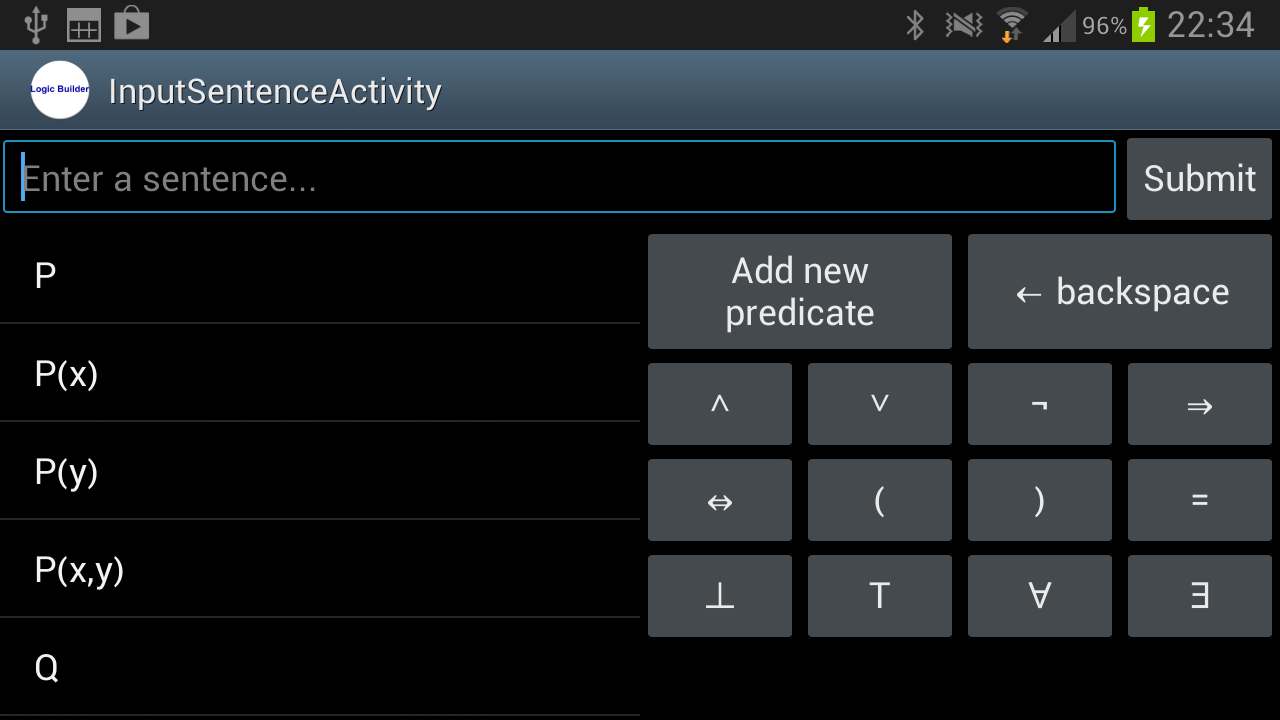
\includegraphics[width=0.9\textwidth]{Images/formulachecker.png}
\caption{User interface for formula checker}
\label{fig:Compilation}
\end{figure}

\subsection{Predictive parsing}

Both disadvantages of top-down parsing mentioned in the previous section can be avoided by creating a predicative parser. This is only possible if the grammar can be transformed into a grammar that belongs to the class LL(k), for some finite integer k. An LL grammar is one which is can be parsed from left to right constructing leftmost derivations.  LL(k) is the class of LL grammars which can deduce the production to use looking only at the next k tokens of input. 

It is possible to define the a property that is both necessary and sufficient for a grammar to be in LL(1). Some definitions are needed first:

\begin{FIRST}

The set FIRST($\alpha$) is the set of terminal symbols that can appear as the first word in some string derived from $\alpha$.
\end{FIRST}
\begin{FOLLOW}
The set FOLLOW($\alpha$) is the set of words that can occur immediately after $\alpha$ in a sentence.
\end{FOLLOW}

\begin{FIRST+}

\[
First^{+} (\text{A} \to \beta) = 
  \begin{cases}
   \text{FIRST(}\beta \text{)} & \text{if } \epsilon \notin \text{FIRST(}\beta \text{)} \\
  \text{FIRST(}\beta \text{)} \cup \text{FOLLOW(A)} & \text{otherwise}
  \end{cases}
\]

\end{FIRST+}

\noindent A grammar can be shown to be in LL(1) iff for all productions of the form A $ \to \beta_1 \mid \ldots \mid \beta_n $ we have: 
\begin{equation}
 First^{+} (A \to \beta_i) \cap First^{+} (A \to \beta_j) = \emptyset \quad \forall \: 1 \le i,j \le n, \: i \not= j 
\end{equation}

\noindent Definitions and further details about the theory of parsing can be found in Engineering a Compiler by Cooper and Torczon. \cite{cooper2011engineering}\\
\\
\noindent As defined earlier, the structure of a well formed formula is: 

$$ \phi := Predicate \mid t_1 = t_2 \mid \phi \land \phi \mid \phi \lor \phi \mid \phi \Rightarrow \phi \mid \phi \Leftrightarrow \phi \mid \forall x \phi \mid \exists x \phi$$


\subsection{Operator precedence}

A decision was made to allow the user to omit unnecessary brackets by using the precedence rules: $\lnot$ binds more tightly than $\land$ and $\lor$, and the latter two bind more tightly than $\Rightarrow$ and $\Leftrightarrow$. Also all binary operators are taken to be right associative so P $\diamond_1$ Q $\diamond_2$ , where $\diamond_1$ and $\diamond_2$ are binary operators from the same precedence level, should be interpreted as (P $\diamond_1$ Q) $\diamond_2$ R  not P $\diamond_1$ (Q $\diamond_1$ R).  

To express the rules of hierarchy a context-free grammar was created  in which non-terminals were added so that reflects the precedence hierarchy of the operators. The idea is simply that each sub-formula of an expression cannot contain an operator of lower precedence unless this sub-formula is surrounded by brackets. 

\begin{equation}
\begin{aligned}
\phi_1 \quad \to& \quad \phi_1 \Rightarrow \phi_1 \quad
\mid \quad \phi_1 \Leftrightarrow \phi_1 \quad
\mid \quad \phi_2
\\
\phi_2 \quad \to& \quad \phi_2 \land \phi_2 \quad 
\mid \quad \phi_2 \lor \phi_2 \quad 
\mid \quad \phi_3 
\\
\phi_3 \quad \to& \quad Predicate \quad
\mid \quad ( \: \phi_1 \: ) \quad
\mid \quad \lnot \phi_3 \quad
\mid \quad \forall \: Var \: \phi_3 \quad
\\ &\mid \quad \exists \: Var \:\phi_3 \quad
\mid \quad Var = Var 
\end{aligned}
\end{equation}
\subsection{Eliminating left recursion}
Grammar 3.2 does not meet property 3.1 for a number of reasons. This particular grammar is both left and right recursive and so is ambiguous. Ambiguous in this sense means that a string can  have more than one distinct parse trees. As mentioned, left-recursive grammars can cause  top-down parsers to enter infinite loops.

Left recursion is also a specific case of a FIRST/FIRST conflict. The reason why is fairly simple. Take any left-recursive production, there is at least one alternative production or the recursion is endless. Clearly, since the left-recursive production has the symbol of the left hand side as the first symbol on the right hand side then it's FIRST set is the union of the FIRST set of all alternative productions. Since the left-recursive production shares elements of it's FIRST set with alternative productions then it is not possible to know which production to use by only looking at the next token of input. 

Many FIRST/FIRST conflicts can be solved using left factoring which is simply the process of taking a non-terminal with multiple productions, factoring out shared prefixes of the alternate productions and inserting a new non-terminal which has the suffixes as it's alternatives.  This process does not always produce an LL(k) grammar since not all grammars have an equivalent LL(k) grammar.

The problem of left recursion can be solved since there exists an algorithm to convert a left recursive grammar into a weakly equivalent right-recursive grammar. Here, weakly equivalent, means that the language they generate are the same. This does not, however, mean that they have the same derivation trees. 

Let  $a_1, a_2, ... ,a_n$  and $b_1, b_2, … ,b_m $ be sequences of terminals and non-terminals where $b_1, b_2, … b_m$  do not start with the non-terminal A. Then for a production of the form:

$$ A \quad \to \quad A a_1 \mid A a_2 \mid \ldots \mid A a_n \mid b_1 \mid b_2 \mid \ldots \mid b_m $$

\noindent We can change this to:


\begin{align*}
A \quad &\to \quad b_1 A' \mid  b_2 A' \mid \ldots \mid b_m A' 
\\ A' \quad &\to \quad a_1  A' \mid a_2  A' \mid \ldots \mid a_n A' \mid ε
\end{align*}


\noindent The result of eliminating left-recursion from grammar 3.2 is:

\begin{equation}
\begin{aligned}
\phi_1 \quad \to& \quad \phi_2 \:\: \phi_1'
\\ \phi_1' \quad \to& \quad \Rightarrow \phi_1\: \phi_1' \quad
\mid \quad \Leftrightarrow \phi_1 \: \phi_1' \quad
\mid \quad \epsilon \quad
\\
\phi_2 \quad \to& \quad \phi_3 \:\: \phi_2'
\\ \phi_2' \quad \to& \quad \land \: \phi_2 \: \phi_2' \quad 
\mid \quad \lor \: \phi_2 \: \phi_2' \quad 
\mid \quad \epsilon \quad
\\
\phi_3 \quad \to& \quad Predicate \quad
\mid \quad ( \: \phi_1 \: ) \quad
\mid \quad \lnot \phi_3 \quad
\mid \quad \forall \: Var \: \phi_3 \quad
\\ &\mid \quad \exists \: Var \:\phi_3 \quad
\mid \quad Var = Var 
\end{aligned}
\end{equation}


\subsection{Resolving FIRST/FOLLOW conflicts}

Grammar 3.3 now has what can be referred to as a  FIRST/FOLLOW conflict. FIRST($\phi_1$) = \{$ \epsilon , \Rightarrow , \Leftrightarrow$\} and  FOLLOW($\phi_1$) = \{ $\Rightarrow, \Leftrightarrow$\}. This creates a conflict on input  $\Rightarrow$ or $\Leftrightarrow$ because $\phi_1$ could be matched by one of these or it could be matched with the empty string and the operator could then be matched the following production. A similar FIRST/FOLLOW conflict is seen for $\phi_2$.

This conflict may be resolved by changing each $\phi_1$, on the RHS of the productions for $\phi_1'$, to the production that is one level higher in the precedence hierarchy i.e. $\phi_2$.  Similarly, change each $\phi_2$, on the RHS of the productions for $\phi_2'$ to $\phi_3$.

Grammar 3.4 shows the result after this conflict has been resolved:

\begin{equation}
\begin{aligned}
\phi_1 \quad \to& \quad \phi_2 \:\: \phi_1'
\\ \phi_1' \quad \to& \quad \Rightarrow \phi_2 \: \phi_1' \quad
\mid \quad \Leftrightarrow \phi_2 \: \phi_1' \quad
\mid \quad \epsilon \quad
\\
\phi_2 \quad \to& \quad \phi_3 \:\: \phi_2'
\\ \phi_2' \quad \to& \quad \land \: \phi_3 \: \phi_2' \quad 
\mid \quad \lor \: \phi_3 \: \phi_2' \quad 
\mid \quad \epsilon \quad
\\
\phi_3 \quad \to& \quad Predicate \quad
\mid \quad ( \: \phi_1 \: ) \quad
\mid \quad \lnot \phi_3 \quad
\mid \quad \forall \: Var \: \phi_3 \quad
\\ &\mid \quad \exists \: Var \:\phi_3 \quad
\mid \quad Var = Var 
\end{aligned}
\end{equation}

Another way to fix the conflict would have been removing each $\phi_1$ from the RHS of $\phi_1'$. Although slightly obscured by the left-factoring, the productions $\phi_1$ and $\phi_2$ would then become right-recursive; more specifically they would have indirect right recursion.

Consequently the operators $\Rightarrow , \Leftrightarrow , \land$ and $\lor$ would become right associative. So a sentence such as P $\lor$ Q $\lor$ R would be accepted by the parser and interpreted as P $\lor$ (Q $\lor$ R), the opposite of what is wanted.  

If both of the changes that were mentioned were implemented the productions would then become non-recursive, meaning that a string such as P $\lor$ Q $\lor$ R would not be recognised by the grammar; brackets would need to be in appropriate places to be recognised by the grammar. This is certainly a usable grammar for FOL. Nevertheless, the aim was to create a more flexible grammar than would infer meaning of using left associativity of binary operators, so it is the alternative that shall be used.

The difference between the grammar 3.4 and the one mentioned above may be subtle but has quite a big effect. Strings of the form P $\diamond_1$ Q $\diamond_2$ R, where $\diamond_1$ and $\diamond_2$ are binary operators from the same precedence level, are now recognised by the grammar, in fact strings of arbitrary length will be accepted provided they keep this structure. No associativity is imposed on the operators at this stage, in the sense that P $\diamond_1$ Q $\diamond_2$ R is not equivalent to either P $\diamond_1$ (Q $\diamond_2$ R) or (P $\diamond_1$ Q) $\diamond_2$ R. This is, nonetheless still progress, as this can easily be corrected when the abstract syntax tree is constructed, which is discussed in section 3.2.7.

\subsection{LL(1) grammar}

It will now be shown that grammar 3.4  belongs to the class LL(1). The end of file will be represented by the symbol \$.

The non-terminal $\phi_1'$ has three alternative productions, the FIRST$^{+}$ set for each of the productions is given below:\\
\\
FIRST$^{+}(\phi_1' \: \to \quad\Rightarrow \phi_2 \phi_1') = \{\Rightarrow \}$\\
FIRST$^{+}(\phi_1' \: \to \quad\Leftrightarrow \phi_2 \phi_1') = \{\Leftrightarrow \}$\\
FIRST$^{+}(\phi_1' \: \to \quad\epsilon) = \{\epsilon, \$, )\}$\\
\\
Each of these sets are disjoint, so the intersection of any two of these sets is the empty set. Similarly, $\phi_2'$ also has three alternative productions, the FIRST$^{+}$  set for these are:\\
\\
FIRST$^{+}(\phi_2' \: \to \quad\lor \phi_3 \phi_2') = \{\lor \}$\\
FIRST$^{+}(\phi_2' \: \to \quad\land \phi_3 \phi_2') = \{\land \}$\\
FIRST$^{+}(\phi_2' \: \to \quad\epsilon) = \{\epsilon, \$,  \Rightarrow, \Leftrightarrow, )\}$\\
\\
Again, the intersection between any pair of these is the empty set. Finally, the only remaining non-terminal with more than one RHS is $\phi_3$, which has 5 alternate productions. The  FIRST$^{+}$  set is given for each: \\
\\
FIRST$^{+}(\phi_3 \: \to \text{Predicate}) = \{\text{Predicate} \}\\$
FIRST$^{+}(\phi_3 \: \to ( \phi_1 )) = \{( \}$\\
FIRST$^{+}(\phi_3 \: \to \lnot \phi_3 ) = \{\lnot \}$\\
FIRST$^{+}(\phi_3 \: \to \forall \text{Var} \phi_3) = \{\forall\}$\\
FIRST$^{+}(\phi_3 \: \to \exists \text{Var} \phi_3) = \{\exists\}$\\

We can see that these 5 sets are all disjoint. So there is no overlap between any FIRST$^{+}$ sets that have the same LHS. Therefore, grammar 3.4 satisfies property 3.1 and so we can conclude that this grammar belongs to the class LL(1).

\subsection{Implementation}

The next choice that had to be made was how the parser itself was to be implemented. The parser could be manually coded or a parser generator could be used. Parser generators take formal description of a language such as a grammar and generates a parser for that language. Many parser generators exist, so to compare the the different options I looked mainly at the following areas:
\begin{description}
\item[Parser class] The classes of parsers than can be generated e.g. LL(1)/ LALR(1).
\item[Output language] The language of the source code of the parser that is generated.
\item[Input notation] The notation that is used to describe the language.
\end{description}

The class of the parsers than can be generated is clearly vital. This is not too much of a constraint since it is known that the grammar is in the class LL(1) which is a subclass of many of the other grammar classes such as LR(1).

For the needs of this project the output language another important feature since it needs to be deployable on the Android platform. The Android platform runs on Dalvik byte-code but code is generally wrote in Java source code which is compiled to Java byte-code and then translated to Dalvik Virtual Machine compatible byte-code automatically. Of course, other languages could be used but this would introduce an extra translation stage between languages which is an unnecessary complication which adds to the complexity and development time. 

Finally, the input notation does not have a strict criteria but should parser generators be equal in other areas then the parser generator with the least complex input notation shall be used.

A manually coded parser could be created in Java that recognises the constructed grammar but this option would require the greatest development time.

After comparing the multitude of parser generators available I opted to use the parser generator JavaCC. JavaCC takes a description of an LL(k) grammar and produces Java source code of a recursive descent parser for that grammar. The description of the grammar is given using Extended Backus-Naur Form. This is similar to the form used so far in this report to describe the different grammars. This simple input notation is a clear benefit of using JavaCC.

Since grammar 3.4 belongs to the class LL(1), JavaCC can generate a predictive parser that has a run time complexity that is linear in terms of the input size.  

\begin{figure}[h]
\centering
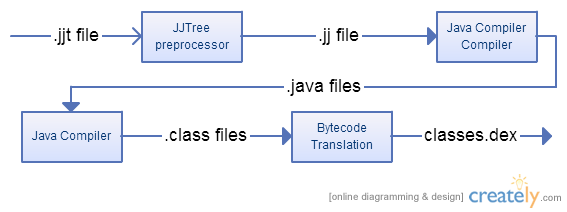
\includegraphics[width=0.9\textwidth]{Images/compilation.png}
\caption{Compilation process for FOL parser}
\label{fig:Compilation}
\end{figure}

\subsection{Abstract Syntax Tree}

In conjunction with JavaCC,  JJTree a JavaCC pre-processor is used. JJTree allows the user to add annotations alongside productions in the grammar which JJTree uses to insert code to the parser that will generate an abstract syntax tree during parsing. 

The AST is generated by creating nodes for terminals first, these will be the leaves of the tree. A tree is built bottom-up with child nodes being assigned as each node is created. The last node to be created will be the root node of the tree. Since each node can have at most two children the resulting AST will be a binary tree.

The following table explains the effect each of the terminals has on the AST.
\\
\begin{tabular}{|l | p{10cm}|}
\hline
Predicate & Each time the parser encounters a Predicate a node is created representing this terminal and this node is then added to a stack. \\ \hline
$\lnot$ &  Node creation is delayed until the next symbol has been fully expanded. Once this has happened the node on the top of the stack is popped and added as a child to the $\lnot$-node which is then itself added to the stack \\ \hline
$\land, \lor, \Rightarrow, \Leftrightarrow, =$ &  As above a node will only be created after the following non terminal has been fully expanded; the two nodes at the top of the stack are then popped and assigned as the children of this node (The grammar guarantees that there will be at least two nodes on the stack at this point). This node is then added to the stack. The process of taking two nodes as soon as the following non-terminal has been fully expanded gives the operators $\land, \lor, \Rightarrow$ and $\Leftrightarrow$ the left associativity that is desired. The = operator does not become left associative as the grammar purposely does not allow it. \\ \hline
$\forall, \exists$ & A similar approach is taken for $\forall$ and $\exists$. The difference here is that $\forall$ and $\exists$ are always followed by a variable. The value of the variable is stored in the same node as the Quantifier. After this the process is the same as for $\lnot$,  once the following symbol has been fully expanded, the node at the top of the stack is added as a child to this one before being added to the stack itself. \\ \hline
Variable & If the variable is following a quantifier then the value of the variable is stored with the quantifier. Otherwise a node is created and added to the stack. \\ \hline
(, ) & No nodes are created for brackets. Brackets can alter the derivation tree of a string, the information conveyed  by any brackets is stored implicitly by the structure of the tree constructed. This has the advantage that regardless of how many brackets the user uses when entering a sentence it will be stored in a consistent manner. \\ \hline
\end{tabular}

\section{Bound and free variables}

When a sentence is being parsed each of the AST nodes that are created for predicates and variables are linked to Java objects representing a predicate or a variable.  This allows two different nodes of the same type to link to the same object. This reflects the way that the same predicate or variable can appear multiple times in a sentence. This is not necessary for any other symbols since each operator has only one interpretation. From here on the words predicate or variable starting with a capital letter will refer to the Java object while the the lower case version will convey the FOL meaning of the word.

A Predicate has two parts: a name and a list of parameters. The name is stored as a string and each parameter is stored as a Variable. 

When a sentence is being parsed, a map of strings to Variables is built. As each predicate is reached the name of each of it's parameters are looked up in the map. If the name is already a key in the map then this argument becomes a reference to the corresponding Variable. If there is no match then a new Variable is created and added to the map. This argument will then refer to this newly created Variable.

When a quantifier is reached a new Variable is created using the variable name given and it is associated with the quantifier.

At the end of parsing all variables in the scope of a quantifier that share the same name as the variable being quantified are bound. This is done as follows: For each predicate in the scope of quantifier, take each argument which has the same name as the quantified variable and set this argument as the Variable associated with the quantifier.

After parsing all variables are either free or bound. If they are free then they point to a Variable that is stored in the map, if they are bound then they point to a Variable associated with a quantifier. This serves as an implicit way of connecting similar Variables. This can be used by rules of inference to easily find all occurrences of a variable, which otherwise would have to traverse the whole tree of a sentence to find each occurrence.

